\chapter{Manipulieren von Bildern}\label{chp:bildmanipulation} %10 Seiten
\glsresetall

 Wie aus Kapitel \ref{chp:bildgenerierung} festzustellen ist, können gute Landschaftsbilder erzeugt werden. Deshalb folgt nun der nächste Schritt, das manipulieren der Bilder. Das Ziel ist es ein Landschaftsbilder zu verschiedenen Tageszeit zu haben, dafür soll der Inhalt der Eingabe beibehalten werden,  der Stile des Bildes sich aber der Tageszeit anpassen. Zum Beispiel aus einem Bild am Tag soll ein Bild bei Nacht werden.
 
 \section{Modelle} % Dani
 Für das manipulieren von Bilder gibt es verschieden Ansätze. Eingegrenzt wurde diese durch den Datensatz, da die Bilder nicht in Paaren vorliegen, es also zu einem Eingabebild keine entsprechendes Bild in der Zieldomain gibt und das Verfahren unsupervised sein soll. %vllt warum unsupervised?
 In Rahmen dieser Arbeit wurden sich mit  zwei Ansätze genauer beschäftigt. Der erste Ansatz ist der des CycleGANs \cite{zhu_unpaired_2020}, welches mittels des cycle consistency losses versucht Bilder zwischen zwei Domänen zu transferieren. Der zweite Ansatz heißt  \gls{acr-funit} \cite{liu_few-shot_2019} der sich am Vorgehen des Menschen Gehirns orientiert und versucht mit wenigen Bilder aus ähnlichen Domänen die Übersetzung zu lernen.
 
 \subsection{CycleGAN}% Dani
 Durch das Fehlen von gepaarten Bilder fehlt eine Möglichkeit zu überprüfen, ob der Generator den Inhalt des Bildes bei behält. \citeauthor{zhu_unpaired_2020} \cite{zhu_unpaired_2020} lösen diese Problem durch einfügen einer weiteren Bedingung: Bilder sollen, wenn sie übersetzt wurden und anschließen wieder zurück umgewandelt werden, gleich sein bzw. sehr ähnlich. Dies wird mittels des cycle consistency loss umgesetzt. 
 Dazu benötigt man zwei GANs, eins welches aus der Eingabedomäne in die Zieldomäne übersetzt, $G: X \rightarrow Y$ und ein anderes welches das Gegenteil durchführt,   $F: Y \rightarrow X$.
 Der cycle consistency loss gibt an wie groß der Verlust zwischen dem ursprünglichen Bild und der Ausgabe nach dem manipulieren beider GANs. 
 Das Ziel ist es $F(G(X))\approx X$ sowie $G(F(Y))\approx Y$ durchzusetzen. Wie in Abbildung \ref{fig:cylce_loss} zusehen, wobei der Verlust jeweils zwischen $x$, $\hat{x}$ und $y$,$\hat{y}$ berechnet wird.
 Die jeweiligen GANs lernen dazu noch über den adversarial loss, also dem Feedback des jeweiligen Discriminators des GANs. 
 Dadurch ergibt sich der Verlust des CycleGANs als
 \[ \mathcal{L}(G,F,D_X,D_Y) = 	\mathcal{L}_{GAN}(G,D_Y,X,Y) + 	\mathcal{L}_{GAN}(F, D_X,Y,X) +\lambda 	\mathcal{L}_{cyc}(G,F)   \]
 wobei $D_X$ und $D_Y$ die Diskriminatoren für die jeweilige Domäne sind und  $\lambda$ die Wichtigkeit des cycle consistency loss festlegt. 
 Das Zeil des Lernens ist es 
 \[G^*,F^* = arg \min_{G,F} \max_{D_X,D_Y} \mathcal{L}(G,F,D_X,D_Y) \] zu lösen.
 
 \begin{figure}
 
 	\tikzstyle{block} = [draw=black, thick, text width=1cm, minimum height=1cm, align=center]  
 	\tikzstyle{line} = [draw=black, thick, text width=1cm, minimum height=3cm, align=center]  
 	\begin{tikzpicture}
 		
 		\node[block] (a) {$x$};
 		\node[block, right=of a] (b) {$\hat{Y}$};
 		\node[block, right=of b] (c) {$\hat{x}$};
 		\node (Dy) [above of=b] {$D_Y$};
 		
 		\node[block, right=of c] (d) {$y$};
 		\node[block, right=of d] (e) {$\hat{X}$};
 		\node[block, right=of e] (f) {$\hat{y}$};
 		\node (Dx) [above of=e] {$D_X$};
 		
 		\path [thick,->,>=stealth]
 		(a) edge [bend left] node [above] {$G$} (b)
 		(b) edge [bend right] node [above] {$F$} (c)
 		(d) edge [bend right] node [above] {$F$} (e)
 		(e) edge [bend left] node [above] {$G$} (f);
 		
 		\draw[dashed,->] (b) to node [] {} (Dy);
 		\draw[dashed,->] (e) to node [] {} (Dx);
 		
 		\draw ([yshift=0.7cm]$(c.north east)!.5!(d.north west)$) --([yshift=-0.7cm]$(c.south east)!.5!(d.south west)$);
 	\end{tikzpicture}
 	\caption[cycle consistency loss]{cycle consistency loss in beide Richtungen}
 	\label{fig:cylce_loss}
 \end{figure}
 
 Durch Evaluierungen und Vergleiche konnten \citeauthor{zhu_unpaired_2020} beobachten, dass die wiederhergestellten Bilder und die echten Bilder ein gute Ähnlichkeit aufwiesen. Vor allem bei Manipulationen bei denen Farben und Texturen geändert werden. Genau diese Veränderungen sollen in dieser Arbeit mit Landschaftsbilder durchgeführt werden. 
 
 \subsection{FUNIT}% Dani
 Der Ansatz von \citeauthor{liu_few-shot_2019} \cite{liu_few-shot_2019}  geht das Problem an, das es oft nicht genug Bilder in der Eingabe- und Zielklassen gibt. Es wurde ein Ansatz mit wenigen Versuche (few-shot) entwickelt. Hierbei wird das Modell mit Bilder aus verschieden Eingabeklassen trainiert und erst beim Testen werden die Bilder der Zielklasse genutzt.
 Dazu wurde eine neues Netzwerkdesign mit dem gegnerischen Training von GANs vereinigt, der Name diese Modells ist  \acrfull{acr-funit}. Dieses Netzwerk besteht aus insgesamt vier Netzen, drei im Generator und eins im Discriminator. Der Generator $G$ bekommt als Eingabe ein Bild $x$ aus der Klasse $C_x$ und ein paar Bilder $y_1,\dots,y_n$ aus einer anderen Eingabeklasse $C_y$. Die Ausgabe $\hat{x}$ sollte dann den Inhalt von Bild $x$ in dem Aussehen der Klasse $K_y$ sein. 
 Die drei Netze die zusammen den Generator ergeben heißen Inhalt Encoder$E_x$, Klassen Encoder $E_y$ und Decoder $F_x$.
 Der Inhalt des Eingabebilds $x$ wird durch den Inhalt Encoder in eine räumliche Feature-Map umgewandelt. Die andern Eingabebilder also  $y_1,\dots,y_n$ werden in den Klassen Encoder gegeben, der  jedes Bild auf eine latenten mittel Vektor ( intermediate latent vector) abbildet und anschließend den Mittelwert über alle Vektoren berechnet, zu sehen in Abbildung \ref{fig:funitmodelsimple}. 
 Mit den Ausgaben aus den beiden Encoder konstruiert der Decoder das Ausgabebild des Generators. 
 \[\hat{x} = G(x, y_1,\dots,y_n)= F_x(E_x(x), E_y(y_1,\dots,y_n))\]
 
 Der Discriminator $D$ hat für jede Klasse die Aufgabe zu entscheiden, ob ein Bild echt ist oder durch den Generator erzeugt wurde. Es wird nur bestraft, wenn bei einem echten Bild nicht die richtige Klasse erkannt wird und wenn ein generierte Bild der Zielklasse zugeordnet wird. Der Generator bekommt nur dann eine Bestrafung, wenn das generiert Bilder nicht der gewünschten Klasse zugeordnet wurde.
 
 Beim Lernen wird das lösen folgender Gleichung versucht:
 
 \[\min_{D} \max_{G} \mathcal{L}_{GAN}(D,G) + \lambda_R \mathcal{L}_R(G) + \lambda_F \mathcal{L}_{F}(G) \]
 
 wobei $ \mathcal{L}_{GAN}(D,G)$ für den Loss des gesamten GANs,$ \mathcal{L}_R(G)$ den der Bildinhaltswiederherstellung und $\mathcal{L}_{F}(G) $ den der Feature-Abstimmung  steht. 
 
 Bei vergleichen mit anderen gängigen Ansätzen schnitt  \gls{acr-funit}  besser ab und benötigt dabei eine kleineren Datensatz \cite{liu_few-shot_2019}. Diese beiden Vorteile bieten sich für die Manipulation die in dieser Arbeit durchgeführt werden soll an.
 
 \begin{figure}[h]
 	\centering
 	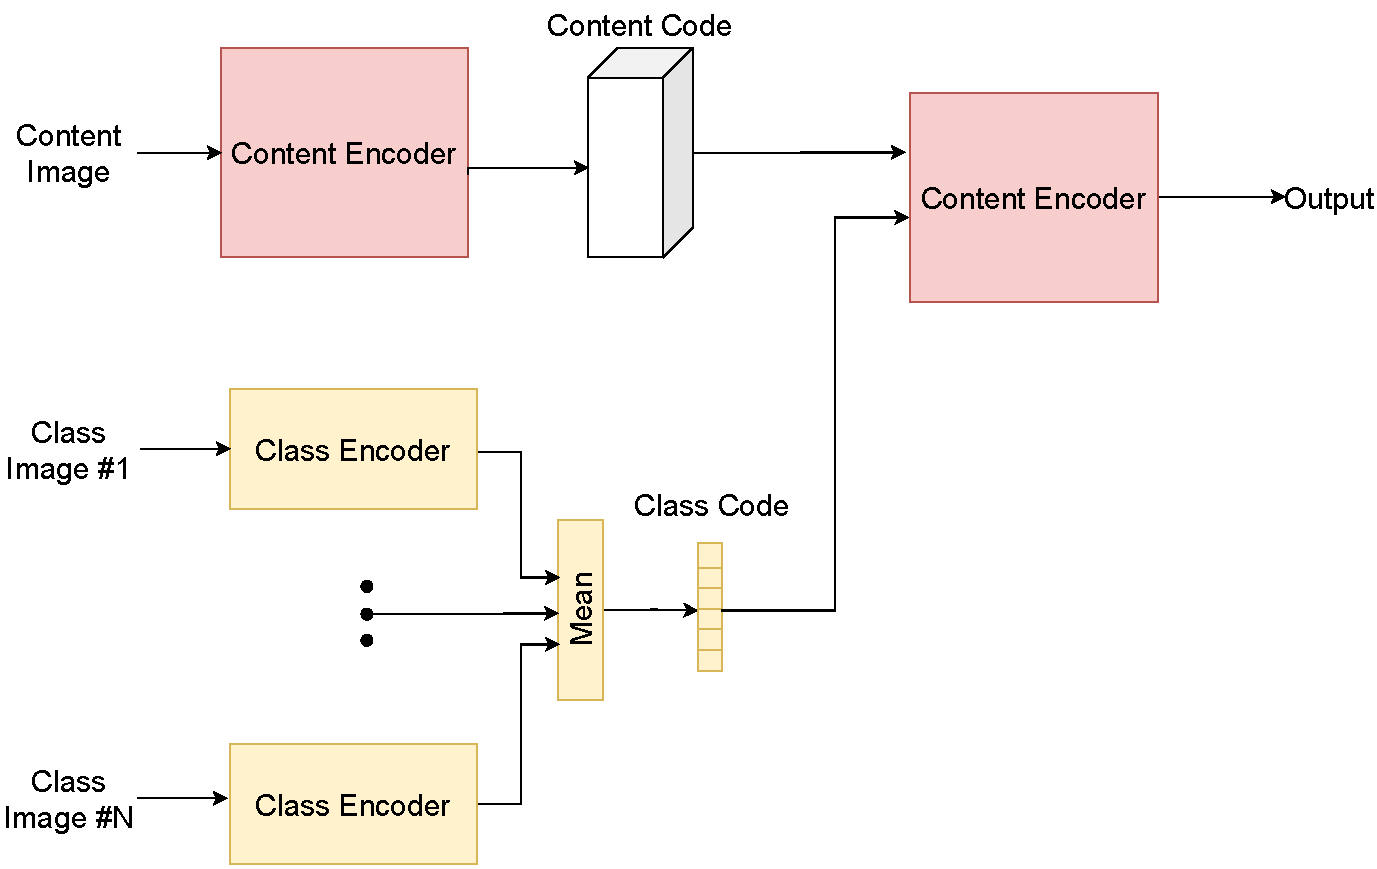
\includegraphics[width=0.8\linewidth]{images/Funit_Model_simple}
 	\caption[Modell FUNIT]{Modell des Generator von FUNIT}
 	\label{fig:funitmodelsimple}
 \end{figure}
 
 
 \section{Implementierung} % Tim nach Implementierung Generieren
 Dieser Abschnitt beschreibt die Implementierung eines CycleGAN. mit Tensorflow und Keras. Da dieses GAN deutlich größer als das \gls{acr-SNDCGAN} ist, konnte es, aufgrund der beschränkten Computerressourcen, nur einmal trainiert werden. Alle Trainingsparameter wurden vorher festgelegt, wobei die Erfahrung aus \cref{sec:gen_impl} 
 
 \subsection{Umsetzung in Tensorflow/Keras}
 Wie auch für das \gls{acr-SNDCGAN} wurde ein \enquote{Sequential model} von Keras~\cite{keras:SequentialModel} verwendet um die einzelnen Schichten abzubilden. Da es nicht alle benötigten Netzschichten in Keras  implementiert sind mussten zudem für die ResBlock und ReflectionPadding2D Schichten, siehe \cref{sub:cyclegan}, sowie für Tanh,  eigene Klassen geschrieben werden, welche von einer abstrakten Keras Schicht erben. 
 
 Das Training des CycleGAN wurde ähnlich wie das \gls{acr-SNDCGAN} in \cref{sec:gen_impl} implementiert. Ebenfalls wurde es durch Checkpoints ermöglicht das Netz jederzeit anzuhalten und später weiter zu trainieren. Adam \cite{tf:adam} wurde als Optimizer, und GradientTapes \cite{tf:gradientape} zur Berechnung der Gradienten, verwendet.
 
Die Optimizer sind identisch parametrisiert und wurden wie in der Implementierung von \cite{brownlee_how_2019-1} auf eine Lernrate von 2e-4 und beta1 auf 0.5 gesetzt. 

Da das CycleGAN aus vier mehrschichtigen Netzen besteht, welche zusammen trainiert werden ist es sehr speicherintensiv zu trainieren. Nur dadurch, dass einzelne Trainingsschritte in eine Funktion mit dem \enquote{tf.function} decorater \cite{noauthor_tffunction_nodate}, ausgelagert sind kann die stärkste dem Projekt zur Verfügung stehende Grafikkarte genug speicher bieten, um das Training mit einer geringen Batchgröße durchzuführen. 


 \section{Evaluierung} % TODO Tim und Joshua

 \paragraph{SIFID} Als Metrik für die Evaluierung der Ergebnisse der
 Bildmanipulation wird die \gls{acr-SIFID} verwendet, die von
 \citeauthor{shaham2019singan} in ihrem Paper \citetitle{shaham2019singan}
 \cite{shaham2019singan} eingeführt wurde. Dies ist eine Erweiterung der bereits
 für die Bildgenerierung verwendeten \gls{acr-FID} \cite{heusel2017gans} (vgl.
 \cref{evalGen} % TODO: Ist die da beschrieben?
 ). Anstatt die Differenz zwischen der Merkmalsverteilung für eine
 Gruppe von generierten und eine Gruppe von originalen Bildern zu messen (so wie
 die \gls{acr-FID}), misst die \gls{acr-SIFID} die Differenz zwischen einem
 Eingabebild in das I2I GAN und dem erzeugen Ausgabebild
 \cite[S. 4575]{shaham2019singan}. Wie die \gls{acr-FID} vergleicht die
 \gls{acr-SIFID} dabei die Aktivierung einer versteckten Schicht des
 \emph{Inception Networks} \cite{szegedy2015going}.
 %TODO: Ist das im Bilderzeugungs-Evaluierungskapitel so vorhanden?
 Anstatt allerdings die
 Aktivierung nach der letzten Pooling-Schicht zu verwenden, nutzt die
 \gls{acr-SIFID} die \enquote{tiefen} Eigenschaften, die in der Aktivierung der
 Convolution-Schicht vor der zweiten Pooling-Schicht zu finden sind \cite[S.
 4575]{shaham2019singan}. Wie für die \gls{acr-FID} sind niedrige Werte besser,
 sie bedeuten, dass der Unterschied zwischen den beiden Bildern geringer ist
 \cite[S. 5]{pang2021image}.